\section{The latent as judge}
\label{sec:judge}

A pretrained JEPA is implicitly an energy over (context, future) pairs,
$E(x, y) = 1 - \cos(\hat{z}(x), \mathrm{enc}([x \,\Vert\, y]))$
\citep{lecun2006ebm}, lowered on true pairs by the invariance term.
Everything below reads it off \emph{frozen} checkpoints.

\begin{figure*}[!t]
\centering
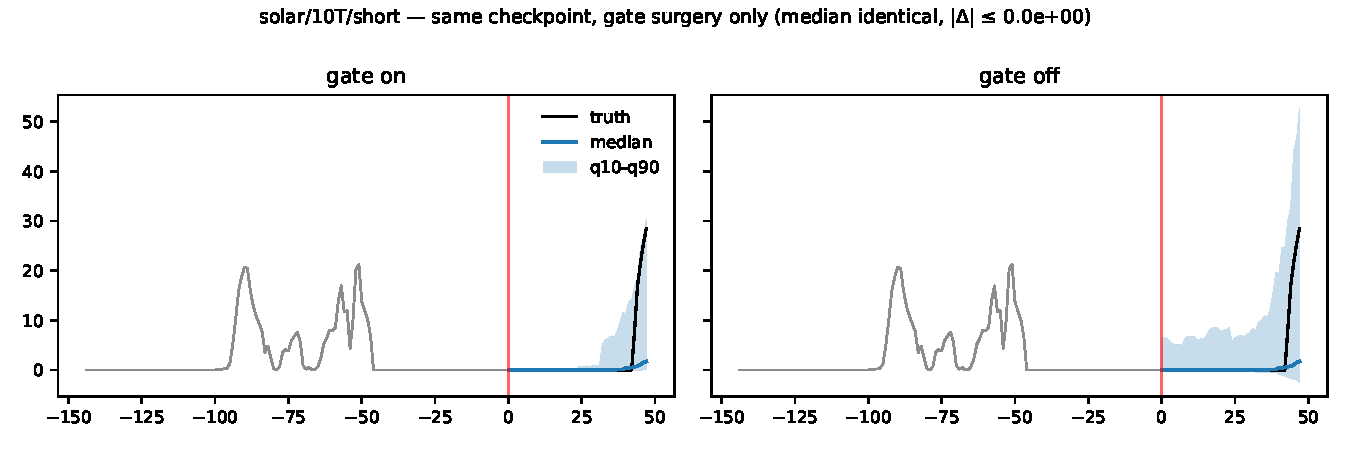
\includegraphics[width=0.92\textwidth]{figures/gate_fan_solar_10T_short.pdf}
\caption{The gate on one solar window (10-minute data), same checkpoint,
same median (max difference $0$), gate surgery only. With the gate, the
fan is pinned to zero through the night, where the outcome is certain,
and opens at sunrise; without it, the same weights spread a worst-case
envelope over certain zeros. Note that the truth briefly escaping the
band at the peak is what a calibrated 80\% interval is supposed to do
one step in five; the gate-off panel that covers everything is the 0.968
coverage pathology of Table~\ref{tab:esjepa} in picture form.}
\label{fig:gatefan}
\end{figure*}


\paragraph{The judge exists; fine-tuning destroys it.}
Figure~\ref{fig:probe}: pretrained checkpoints rank the true future at
0.21--0.25 among 34 candidates (chance 0.50; median rank 0.000 on hourly
electricity for the best judge), while a fully fine-tuned checkpoint
degrades to 0.41. The judge peaks early in pretraining and erodes while validation keeps
improving, so judge selection uses an early probe; it also scales with
capacity faster than forecasting does.

\begin{figure}[t]
\centering
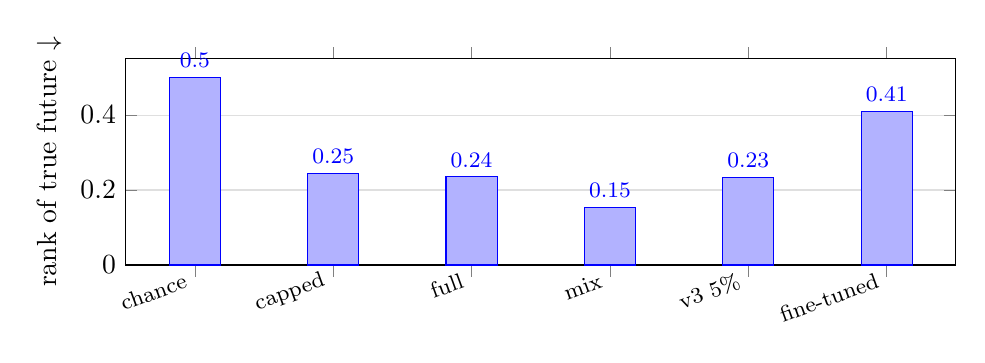
\begin{tikzpicture}
\begin{axis}[
  width=\columnwidth, height=4.2cm, ybar,
  ymin=0, ymax=0.55,
  ylabel={rank of true future $\downarrow$},
  symbolic x coords={chance, capped, full, mix, v3 5\%, fine-tuned},
  xtick=data, x tick label style={rotate=20, anchor=east, font=\footnotesize},
  bar width=6.5mm, ymajorgrids, grid style={gray!25},
  nodes near coords, every node near coord/.append style={font=\footnotesize}]
\addplot coordinates {(chance,0.50) (capped,0.245) (full,0.235)
  (mix,0.153) (v3 5\%,0.233) (fine-tuned,0.409)};
\end{axis}
\end{tikzpicture}
\caption{The judge lives in the pretrain and dies in the fine-tune
(normalized rank of the truth among 34 candidates; 0.50 is chance).}
\label{fig:probe}
\end{figure}

\paragraph{A zero-training reranker that upgrades TTM-R3
(Table~\ref{tab:hybrid}).}
Candidate futures are scored with $E$ and read out as weighted
quantiles; candidates share the proposer's center, and degenerate pools
fall back to uniform weights (pool design, and the four-fold dilution
replication that forced it, in Appendix~\ref{app:training}).

\begin{table}[t]
\centering
\scriptsize
\begin{tabular}{lcccccc}
\toprule
WQL vs SN $\downarrow$ & ettm1 & ettm2 & etth1 & etth2 & weather & exch. \\
\midrule
TTM-R3 alone & 0.88 & 0.81 & 0.85 & 0.95 & \textbf{0.63} & 0.88 \\
+ judge (centered) & \textbf{0.77} & \textbf{0.72} & \textbf{0.71} & \textbf{0.78} & 0.64 & \textbf{0.78} \\
\bottomrule
\end{tabular}
\caption{A frozen 1M judge turns a point forecaster into a probabilistic
one that beats or ties its own WQL on 6/6 held-out datasets, zero
additional training, replicated across judges from two pretraining
lineages. On all 97 GIFT configurations (paired windows) the pipeline
beats TTM's collapsed point CRPS by 7\% at a 3.8\% MASE tax; coverage
(0.62 vs 0.80 nominal) is the open gap. Given a deliberately biased
proposer, the judge moves its mass to the alternative center it keeps in
the pool: a verifier that can fire its proposer.}
\label{tab:hybrid}
\end{table}

\paragraph{Four dimensions carry the calibration
(Table~\ref{tab:esjepa}).}
\label{sec:esjepa}
The predictor converges to a conditional mean
(Section~\ref{sec:architecture}); rather than the residual, irrecoverable
by definition, a 4-D head predicts its \emph{statistics} (log-RMS,
log-MAD, skewness, lag-1 autocorrelation around a causal EWMA),
deterministic functions of the data, so nothing can collapse. Predicted
volatility correlates with realized at 0.63, against 0.3--0.4 for the
signal path: volatility is more predictable than its realization.
Figure~\ref{fig:gatefan} shows the mechanism on one window.

\begin{table}[!t]
\centering
\scriptsize
\begin{tabular}{lccc}
\toprule
Configuration (flip) & CRPS & 80\% cov. & MASE \\
\midrule
champion, no z & \textbf{0.596} & 0.769 & 0.870 \\
z arm, best ckpt & 0.598 & 0.790 & 0.874 \\
z arm, early ckpt & 0.626 & \textbf{0.800} & 0.921 \\
\quad gate bias $\to 0$ & 0.626 & 0.813 & 0.921 \\
z arm, \emph{gate off} & 0.785 & 0.968 & 0.873 \\
\bottomrule
\end{tabular}
\caption{Residual-statistics ablations by evaluation-time weight
surgery. Gate off: $+18.7$ CRPS points, coverage exploding, MASE moving
by less than $10^{-3}$ (median invariance verified in production).
Fine-tuning co-adapted the organs: base widths converge to a worst-case
envelope, the gate to conditional sharpening; four latent dimensions
carry the calibration. The counterfactual trained without z is the
champion at 0.596: z buys nominal coverage at equal CRPS.}
\label{tab:esjepa}
\end{table}
